\documentclass[a4paper]{article}
\usepackage[utf8x]{inputenc}
\usepackage[T1,T2A]{fontenc}
\usepackage[russian]{babel}
\usepackage{hyperref}
\usepackage{indentfirst}
\usepackage{listings}
\usepackage{color}
\usepackage{here}
\usepackage{array}
\usepackage{multirow}
\usepackage{graphicx}
\usepackage{caption}
\graphicspath{{graphics/}}
\usepackage[left=2cm,right=2cm,
top=2cm,bottom=2cm,bindingoffset=0cm]{geometry}
\usepackage{listings}
\lstset{ %
	extendedchars=\true,
	keepspaces=true,
	language=bash,					% choose the language of the code
	basicstyle=\footnotesize,		% the size of the fonts that are used for the code
	numbers=left,					% where to put the line-numbers
	numberstyle=\footnotesize,		% the size of the fonts that are used for the line-numbers
	stepnumber=1,					% the step between two line-numbers. If it is 1 each line will be numbered
	numbersep=5pt,					% how far the line-numbers are from the code
	backgroundcolor=\color{white},	% choose the background color. You must add \usepackage{color}
	showspaces=false				% show spaces adding particular underscores
	showstringspaces=false,			% underline spaces within strings
	showtabs=false,					% show tabs within strings adding particular underscores
	frame=single,           		% adds a frame around the code
	tabsize=2,						% sets default tabsize to 2 spaces
	captionpos=b,					% sets the caption-position to bottom
	breaklines=true,				% sets automatic line breaking
	breakatwhitespace=false,		% sets if automatic breaks should only happen at whitespace
	escapeinside={\%*}{*)},			% if you want to add a comment within your code
	postbreak=\raisebox{0ex}[0ex][0ex]{\ensuremath{\color{red}\hookrightarrow\space}}
}

\begin{document}	% начало документа

\begin{titlepage}	% начало титульной страницы

	\begin{center}		% выравнивание по центру

		\large Санкт-Петербургский Политехнический Университет Петра Великого\\
		\large Институт компьютерных наук и технологий \\
		\large Кафедра компьютерных систем и программных технологий\\[6cm]
		% название института, затем отступ 6см
		
		\huge Телекоммуникационные технологии\\[0.5cm] % название работы, затем отступ 0,5см
		\large Отчет по лабораторной работе №2 \\[0.2cm]
		\large\textbf{"Ряд Фурье. Преобразование Фурье. Корреляция"}\\[5cm]

	\end{center}


	\begin{flushright} % выравнивание по правому краю
		\begin{minipage}{0.25\textwidth} % врезка в половину ширины текста
			\begin{flushleft} % выровнять её содержимое по левому краю

				\large\textbf{Работу выполнила:}\\
				\large Власова А.В.\\
				\large {Группа:} 33501/4\\
				
				\large \textbf{Преподаватель:}\\
				\large Богач Н.В.\

			\end{flushleft}
		\end{minipage}
	\end{flushright}
	
	\vfill % заполнить всё доступное ниже пространство

	\begin{center}
	\large Санкт-Петербург\\
	\large \the\year % вывести дату
	\end{center} % закончить выравнивание по центру

\thispagestyle{empty} % не нумеровать страницу
\end{titlepage} % конец титульной страницы

\vfill % заполнить всё доступное ниже пространство

\section{Цель работы}
Получить представление о спектрах телекоммуникационных сигналов.

\section{Постановка задачи}
\begin{itemize}
	\item Для сигналов, построенных в лабораторной работе №1, выполнить расчет преоразования Фурье. Перечислить свойства преобразования Фурье.
	\item С помощью функции корреляции найти позицию синхропосылки [101] в сигнале [0001010111000010]. Получить пакет данных, если известно, что его длина составляет 8 бит без
	учета синхропосылки. Вычислить корреляцию прямым методом, воспользоваться алгоритмом быстрой корреляции, сравнить время работы обоих алгоритмов.
\end{itemize}

\section{Теоретический раздел}
\subsection{Свойства преобразования Фурье}
Основные свойства преобразования Фурье (ПФ):
\begin{enumerate}
	\item Суммирование функций\\
    ПФ линейной комбинации некоторых функций равно аналогичной линейной комбинации ПФ этих функций.
    \item Смещение функции\\
    При смещении функции по аргументу на $t_0$ ее ПФ умножается на $e^{j2{\pi}ft_0}$.
    \item Изменения масштаба аргумента функции\\
    Если аргумент функции $y(t)$ заменить на $at$, где $a$ -- постоянный коэффициент, то ПФ с $Y(f)$ изменится на $\frac{1}{|a|}Y(\frac{f}{a})$.
    \item Перемножение функций\\
    ПФ произведения двух функций равно свертке их ПФ:
    $F[x(t)y(t)]={\frac{1}{2{\pi}}}[X(f)*Y(f)]$
    \item Свертывание функций\\
    ПФ свертки двух функций равно произведению ПФ свертываемых функции: $F[x(t)*y(t)]=X(f)Y(f)$
    \item Дифференцирование функции\\
    При дифференцировании функции $y(t)$ ее ПФ умножается на $j2{\pi}f$.
    \item Интегрирование функции\\
    При интегрировании от $-{\infty}$ до $t$ функции, имеющей равную нулю постоянную составляющую, ее ПФ делится на $j2{\pi}f$.
    \item Обратимость\\
    ПФ обратимо с точностью до знака аргумента.
\end{enumerate}
\subsection{Корреляция}
Корреляция используется для того, чтобы определить степень независимости одного процесса от другого или установить сходство одного набора данных с другим.
Дискретной кросс-корреляцией функций $f(t)$ и $g(t)$ называется следующая операция:\\\\
$corr(f,g)[n] = {\sum_{m=-{\infty}}^{\infty}}f(m)g(n+m)$\\\\
, где $m$ -- величина задержки. \\\\
Кросс-корреляция чаще всего применяется в обработке сигналов, при этом $f$ считается образцом, а $g$ -- сигналом, содержащим образец. Результат -- это вектор чисел, показывающих, насколько сильно образец выражен в сигнале.\\
Расчет корреляции можно ускорить, используя теорему о корреляции, которая формулируется следующим образом:\\\\
$r_{12}(j)={\frac{1}{N}}F_D^{-1}[X(k)Y(k)]$\\\\
, где $F_D^{-1}$ обозначает обратное дискретное преобразование Фурье. Данный подход требует выполнения двух дискретных пробразований Фурье и одного обратного, что легче всего сделать, используя алгоритм БПФ. Если число членов в последовательностях достаточно велико, данный метод БПФ дает результат быстрее, чем непосредственный расчет взаимной корреляции. 

\section{Ход работы}
Для нахождения позиции синхропосылки в сигнале воспользуемся алгоритмами кросс-корреляции и быстрой корреляции. Сгенерируем сигнал [0001010111000010] и синхропосылку [101].
\center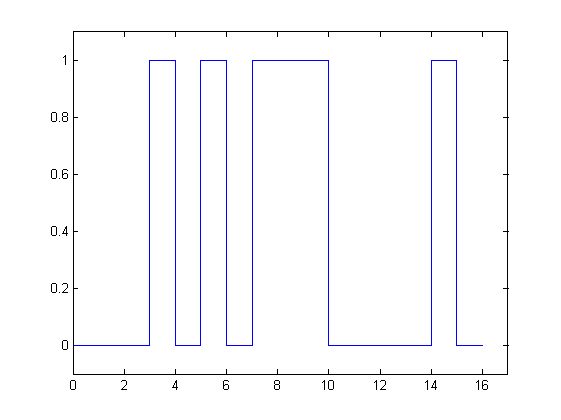
\includegraphics[scale = 0.7]{signal.png} \\ Рис. 1 Исходный сигнал \\ 

\flushleft Выполним кросс-корреляцию с помощью функции xcorr.
\captionof{lstlisting}{Кросс-корреляция}
\lstinputlisting[firstline=20, lastline=22]{../lab2.m}
\center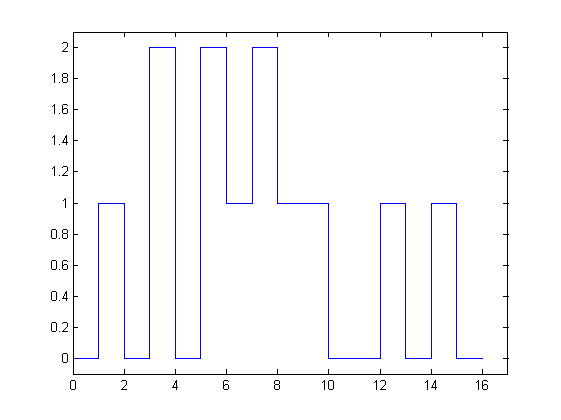
\includegraphics[scale = 0.7]{xcorr.png} \\ Рис. 2 Результат выполнения кросс-корреляции \\

\flushleft Применим алгоритм быстрой корреляции.
\captionof{lstlisting}{Быстрая корреляция}
\lstinputlisting[firstline=25, lastline=30]{../lab2.m}
\center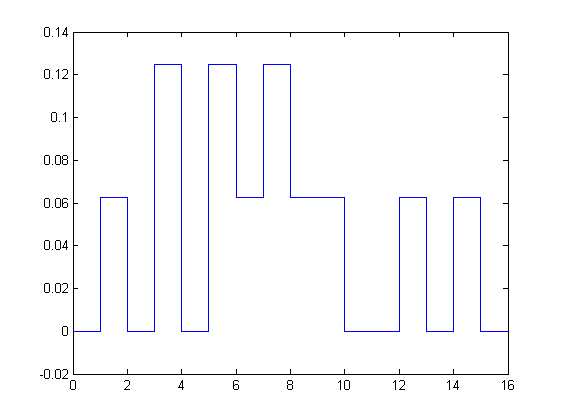
\includegraphics[scale = 0.7]{fast.png} \\ Рис. 3 Результат выполнения быстрой корреляции \\

\flushleft Сравим время работы двух алгоритмов для случайных сигналов длины N.\\
\flushright Таблица 1
\begin{center}
	\begin{tabular}{|p{3cm}|p{3cm}|p{3cm}|}
		\hline N&$t_{xcorr}$,c&$t_{fast}$,c \\
		\hline 50&0.000403&0.0000279 \\
		\hline 100&0.000422&0.0000474 \\
		\hline 500&0.000533&0.0000762 \\
		\hline 1000&0.000623&0.00012 \\
		\hline 5000&0.0021&0.0005126 \\
		\hline 10000&0.0035&0.0010 \\
		\hline 50000&0.0198&0.0056 \\
		\hline 100000&0.1520&0.0887 \\
		\hline 500000&0.2824&0.1293 \\
		\hline 
	\end{tabular}
\end{center}
~\
\flushleft Для сигналов небольшой длины алгоритм быстрой корреляции работает примерно в 10 раз быстрее кросс-корреляции, для сигналов длиной от 50000 - в 2 раза быстрее.  

\section{Выводы}
Преобразование Фурье является математической основой спектрального анализа сигналов, который, в свою очередь, находит широкое применение в телекоммуникационных технологиях. Например, государственные регулирующие структуры распределяют различные частоты для разных радио-служб: телевизионное и радиовещание, сотовая связь, связь правоохранительных органов и спасательных служб, а также множество других организаций и приложений. Важно, чтобы каждая служба работала на предназначенной для нее частоте и оставалась в пределах выделенной полосы канала. 
\end{document}



